%
% achromat.tex
%
% (c) 2019 Prof Dr Andreas Müller, Hochschule Rapperswil
%
\subsection{Achromat\label{mo:subsection:achromat}}
Die meisten Medien brechen Licht unterschiedlicher Wellenlängen
verschieden stark.
Bei einer einzelnen Linse führt dies dazu, dass die Farben
verschieden grosse Brennweite haben.
Dies führt zu unschönen Farbsäumen und unscharfer Abbildung.

Die Abhängigkeit der Brechkraft von der Wellenlänge heisst {\em Dispersion}.
\index{Dispersioin}
Es gibt zwar auch Gläser mit sehr geringer Dispersion, doch sind diese
leider sehr teuer in der Herstellung und zum Teil auch empfindlich
auf Umwelteinflüsse.
Calzium-Fluorit zum Beispiel hat fast verschwindende Dispersion, darf
aber keinen grossen Temperaturveränderungen ausgesetzt werden.
Es wird daher nur in Spezialanwendungen eingesetzt, zum Beispiel bei
der Masken-Belichtung in der Chip-Herstellung oder für hochwertige 
Astrographen.

Da es Gläser ganz unterschiedlicher Dispersion gibt, besteht die Hoffnung,
durch Kombination geeigneter Gläser in einem mehrlinsigen System zu
erreichen, dass die Farben rot und blau die gleiche Brennweite haben.
Die Farbe grün dazwischen kann dann auch nicht allzu weit weg sein.
Auf diese Art erhält man ein System mit deutlich schwächeren Farbrändern
und grösserer Bildschärfe.

Das einfachste solche System ist der Achromat, erfunden vom  englischen
Amateuroptiker Chester Moor Hall im Jahre 1733 (Abbildung~\ref{mo:achr}).
Eine Sammellinse aus Kronglas wird mit einer Zerstreuungslinse aus
Flintglas zusammengefügt.
Es entsteht ein System mit drei gekrümmten Flächen, deren Abstand
in begrenztem Rahmen gewählt werden kann.
Es stehen also insgesamt fünf Parameter zur Verfügung, die so gewählt
werden müssen, dass rotes und grünes Licht die gleiche Brennweite
erhalten.

\subsubsection{Konstruktion}
In diesem Abschnitt soll ein Achromat aus Kron- und Flintglass
mit einer vorgegebenen Brennweite von $f=200\,\text{mm}$ 
entwickelt werden.
In Abbildung~\ref{mo:achr} ist die Anordnung der Linsen des
Achromaten dargestellt.
Im Laufe der Entwicklung sind die Unbekannten $R_1$, $R_2$, $R_3$, $d_1$
und $d_2$ so zu bestimmen, dass der Achromat für rot und grün die
gleiche Brennweite hat.

\begin{figure}
\centering
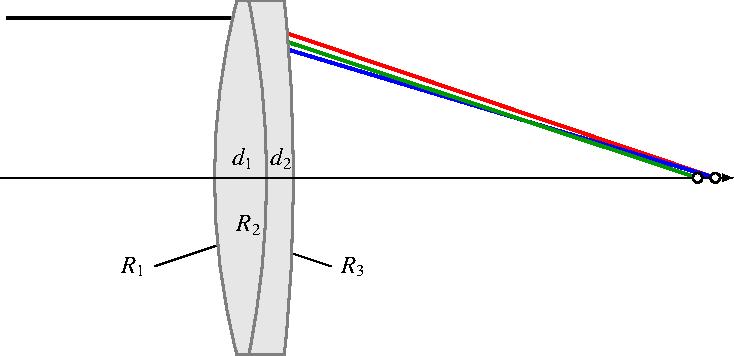
\includegraphics{applications/matrixoptik/achr.pdf}
\caption{Ein Achromat besteht aus einer Sammellinse aus Kronglas und einer
Zerstreuungslinse aus Flintglas.
Dank der verschiedenen Brechungsindizes dieser beiden Gläser für rotes
und grünes Licht fokusiert das System rotes und blaues Licht in den gleichen
Brennpunkt und vermeidet damit Farbränder und verbessert die Abbildungschärfe.
\label{mo:achr}}
\end{figure}

Auf der Website \url{https://refractiveindex.info} kann man detaillierte
Informationen über den Brechungsindex sehr vieler kommerziell erhältlicher
optischer Gläser.
Wir entnehmen ihr die Daten in Tabelle~\ref{mo:indextabelle} für Kron-
und Flint-Glas, genauer für die Gläser SCHOTT-K und SCHOTT-F des Herstellers
SCHOTT AG in Mainz.
\begin{table}
\centering
\begin{tabular}{|l|r|r|r|}
\hline
Farbe&Wellenlänge&Kronglas $n_1$&Flintglas $n_2$\\
\hline
rot  &700nm& 1.507&1.612\\
grün &550nm& 1.513&1.623\\
blau &450nm& 1.519&1.638\\
\hline
\end{tabular}
\caption{Brechungsindizes von Kron- und Flintglass (Schott K und Schott F)
für verschiedene Farben
\label{mo:indextabelle}}
\end{table}

\subsubsection{Die Transfergleichungen}
Das in Abbildung~\ref{mo:achr} dargestellte System hat die
Transfer-Matrix
\begin{align*}
T
&=
T_f
B(n_2,1,R_3)
T_{d_2}
B(n_1,n_2,R_2)
T_{d_1}
B(1,n_1,R_1).
\\
&=
\begin{pmatrix}1&f\\0&1\end{pmatrix}
\begin{pmatrix} 1&0\\\frac{1}{R_3}\left(n_2-1\right)&n_2\end{pmatrix}
\begin{pmatrix}1&d_2\\0&1\end{pmatrix}
\begin{pmatrix} 1&0\\\frac{1}{R_2}\left(\frac{n_1}{n_2}-1\right)&\frac{n_1}{n_2} \end{pmatrix}
\begin{pmatrix}1&d_1\\0&1\end{pmatrix}
\begin{pmatrix} 1&0\\\frac{1}{R_1}\left(\frac{1}{n_1}-1\right)&\frac{1}{n_1} \end{pmatrix}
\end{align*}
Aus der Transfermatrix erhalten wir eine Gleichung dadurch, dass der
achsenparallele Strahl in der Höhe $y$ im Brennpunkt die Höhe $0$ hat.
Dies bedeutet, dass
\[
T\begin{pmatrix}y\\0\end{pmatrix}
=
yTe_1
=
\begin{pmatrix}0\\?\end{pmatrix}
\qquad\text{mit}\qquad
e_1 = \begin{pmatrix}1\\0\end{pmatrix}
\]
sein muss.

Beim Ausmultiplizieren der Matrix $T$ entstehen sehr komplizierte Ausdrücke,
deren Lösung nicht besonders instruktiv ist.
Wir vereinfachen daher das Problem durch zwei Massnahmen:
\begin{enumerate}
\item Wir gehen davon aus, dass die zweite Linse keine Krümmung in Richtung
zum Brennpunkt hat (sogenannte Plano-Linse).
Diese bedeutet das $R_3=\infty$ und damit
\[
B(n_2,1,\infty)= \begin{pmatrix} 1&0\\0&n_2\end{pmatrix}.
\]
\item
Wir geben die Abstände $d_1=5\,\text{mm}$ und $d_2=1\,\text{mm}$ vor.
\end{enumerate}
Mit diesen Vereinfachungen müssen nur noch die beiden Krümmungen $R_1$ 
und $R_2$ bestimmt werden.

Mit einem Computer-Algebra-Programm kann man die erste Komponente von $Te_1$ 
berechnen.
In die entstehenden Ausdrücke kann man die bekannten Werte von
$d_1$ und $d_2$ einsetzen.
Indem man die Werte für $n_1$ und $n_2$ für rot und blau einsetzt, 
erhält man zwei quadratische Gleichungen für $R_1$ und $R_2$.
Die Gleichungen haben zwei Lösungen, aber nur die Kombination
\begin{equation}
\begin{aligned}
R_1&=\phantom{-} 85.41331670548975,
\\
R_2&=-95.89206695802633
\end{aligned}
\label{mo:solution:radii}
\end{equation}
lassen sich als Linsensystem realisieren.
\begin{figure}
\centering
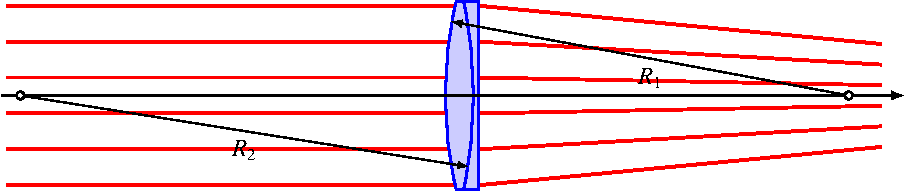
\includegraphics[width=\hsize]{applications/matrixoptik/solution.pdf}
\caption{Masstabgetreue Darstellung der Lösung des Achromat Problems
mit den Krümmungsradien von
\eqref{mo:solution:radii}.
\label{mo:solution:image}}
\end{figure}
Diese Lösung ist massstabsgetreu in Abbildung~\ref{mo:solution:image}
dargestellt.
Dieser Achromat ist mit einem Linsendurchmesser von 4\,cm ist realistisch
herstellbar.

\subsubsection{Brennweite für grün}
Die oben in \eqref{mo:solution:radii} gefundene Lösung kann man jetzt
zusammen mit den Werten von $n_1$ und $n_2$ für grün und $d_1$ und $d_2$
in den Ausdruck für $T$ einsetzen und wie im
Abschnitt~\ref{mo:subsection:linse} die Brennweite des Systems für die
Farbe grün berechnen.
Wie erwartet ist die Brennweite für grün kürzer, nämlich
\[
f_{\text{grün}} = 199.163\,\text{mm}.
\]

Gehen wir von einem Linsendurchmesser von 4\,cm aus, dann ist der Durchmesser
$d$
des roten bzw.~blauen Strahlenkegels bei der Brennweite $f_{\text{grün}}$
durch den Strahlensatz geben:
\[
4\,\text{cm} : f = d : (f - f_{\text{grün}})
\qquad \Rightarrow \qquad
d = \frac{40}{200}\cdot (200-199.163) = \frac15\cdot 0.837 = 0.1674\,\text{mm}.
\]
Genau in der Mitte zwischen den beiden Brennpunkten $f$ und $f_{\text{grün}}$
kann man also mit dem kleinstmöglichen ``Brennfleck'' mit einem Durchmesser
von $0.084\,\text{mm}$ rechnen.
Ein typischer CMOS-Sensor hat einen Pixeldurchmesser von etwa $5\,\mu\text{m}$,
der Brennfleck ist also 17mal grösser als ein Pixel.
Dieser Achromat ist also viel zu wenig präzise für einen modernen CMOS-Sensor.





